\documentclass[11pt, a4paper]{article}
\usepackage{amsmath}
\usepackage{graphicx}

\title{Versuch 1: Akustik}
\author{Jascha Fricker, Benedict Brouwer}

\begin{document}
    \maketitle

    \section{Abstract}
    In diesem Versuch wird die Schallgeschwindigkeit in verschiedenen elastischen Medien
    duch verschieden Versuchsaufbauten bestimmt.

    \tableofcontents

    \newpage
    
    \section{Theorie}
    Schall breitet sich in Form einer Welle aus. Diese Welle kann mit der Funktion
    \begin{align}
        a(x, t) = A \cdot cos(\omega t-kx+\phi )
    \end{align}
    beschrieben werden. Mit dieser Formel kann die Phasengeschwindugkeit
    \begin{align}
        \nu = \frac{\lambda}{T} = \frac{\omega}{k} = f \cdot \lambda
    \end{align}
    hergeleitet werden. \\
    \section{Phasengeschwindigkeit in Festkörpern}

    \subsection{Theorie und experiemteller Aufbau}
    In Aufgabe 1 wird die Phasengeschwindigkeit einer longitundinalen Welle in elastischen Festkörpern (Staben aus verschiedenen Materialien) bestimmt.
    Nachdem diese am oberen Ende angeschlagen wurden, laufen die Wellenpackete entlang des Stabes und werden an den Enden reflektiert.
    Durch ein Piezoelement kann an einem Ende mit einem Oszilloskop ein Ausschlag gemessen werden, wenn eine Welle ankommt.
    Mithilfe der Differenz dieser Ausschläge kann dann die Phasengeschwindigkeit berechnet werden. Es gilt
    \begin{align}
        \nu = \frac{2l}{t} \ ,
    \end{align}
    da die Welle zweimal die Stablänge zurücklegt. Mit dieser und der Formel für longitundinale Wellen
    \begin{align}
        \nu = \sqrt{\frac{E}{\rho}}
    \end{align}
    kann das Elastizitätsmodul des Materials
    \begin{align}
        \nu = \frac{2l}{t} = \sqrt{\frac{E}{\rho}} \ \ \Rightarrow \ \ E = 4\frac{l^2}{t^2} \rho
    \end{align}
    berechnet werden.

    \subsection{Ergebnisse}
    \subsubsection{Messwerte}
    Zu jedem Material wurde ein mehrmals der Abstand des ersten zum
    vierten Peak gemessen, um die Genauigkeit zu vergrößern. Da die Messwerte aber immer im Fehlerbereich lagen,
    wird zu vereinfachung der Auswertung immer nur ein Messwert betrachtet. Dieser ist in Tabelle \ref{ex:mess1}
    angegeben. 
    \begin{table}[]
        \centering
        \begin{tabular}{c | c | c | c}
           & Messig & Kupfer & Aluminium \\ \hline
            $ t $ für 4 Peaks & $ 2480(6)ms $ & $ 2360(6)ms $ & $ 1800(6)ms $ \\ \hline
            Länge $l$ des Stabs & $1407(14)mm$ & $1501(14)mm$ & $1502(14)mm$ \\ \hline
            Elastizitätsmodul & $99,7(3,3)\frac{kN}{mm^2}$ & $130,3(3,3)\frac{kN}{mm^2}$ & $67,7(3,3)\frac{kN}{mm^2}$ \\ \hline
            Literaturwert & $78-123\frac{kN}{mm^2}$ & $120\frac{kN}{mm^2}$ & $70\frac{kN}{mm^2}$
        \end{tabular}
        \caption{Messwerte der Zeitdifferenz der Peaks und Länge der  Stäbe}
        \label{ex:mess1}
    \end{table}
    \subsubsection{Messunsicherheiten}
    \paragraph{Zeitmessung}
    Das Oszilloskop misst die Zeit mit einer Cursorgenauigkeit von $ 20ms $. Da das Oszilloskop digital ist, wird
    eine rechteckige Zufallsverteilung angenommen.
    \begin{align}
        a = 20ms \ \Rightarrow \ u_{Cursor}(t) = \frac{a}{2 \sqrt{3}} = \frac{10}{\sqrt{3}}ms
    \end{align}
    Da die Differenz jedoch mit zwei Cursor gemesser wird, gilt:
    \begin{align} \label{eqt}
        u_{t}(t) = \sqrt{2} \cdot u_{Cursor}(t) = \sqrt{10\frac{2}{3}}ms
    \end{align}
    \paragraph{Länge}
    Die Länge wurde mit einem Zollstock gemessen. Im Aufgabenblatt wird die Herstellungsgenauigkeit
    \begin{align}
        u_H(l) = a+b \cdot L = 0,6mm + 0,4\frac{mm}{m} \cdot L = 1,4mm
    \end{align}
    angegeben, da L bei Messing Kupfer und Aluminium $2m$ ist.
    Für die Ablesegenauigkeit gilt
    \begin{align}
        u_A(l) = \frac{a}{2\sqrt{6}} = \frac{1}{2\sqrt{6}}mm,
    \end{align}
    da der Zollstock jeden Millimeter ein Strich hat und eine Dreiecksverteilung angenommen wird.
    Daraus folgt:
    \begin{align} \label{eql}
        u_l = \sqrt{u_H(l)^2 + u_A(l)^2} = \sqrt{\frac{173}{120}}mm
    \end{align}

    \paragraph{Fehlerfortpflanzung}
    Es gilt:
    \begin{align}
        E = 4\frac{l^2}{\frac{t}{3}^2} \rho \\
    \end{align}
    daraus folgt:
    \begin{align}
        u(\bar{E}) &= \sqrt{\left[\frac{\partial E}{\partial t}\right]^2_{\bar{l}, \frac{\bar{t}}{3}, \bar{\rho}} u_{t}(\bar{t})^2 +
        \left[\frac{\partial E}{\partial l}\right]^2_{\bar{l}, \bar{t}, \bar{\rho}} u_{l}(\bar{l})^2 +
        \left[\frac{\partial E}{\partial \rho}\right]^2_{\bar{l}, \bar{t}, \bar{\rho}} u_{\rho}}(\bar{\rho})^2 \nonumber \\
        &= \sqrt{64 \frac{\bar{l}^4 \bar{\rho}^2}{\frac{\bar{t}}{3}^6} \cdot u_t(\bar{t})^2 +
        64 \frac{\bar{l}^2 \bar{\rho}^2}{\frac{\bar{t}}{3}^4} \cdot u_l(\bar{l})^2 +
        16 \frac{\bar{l}^4}{\frac{\bar{t}}{3}^4} \cdot u_{\rho}(\bar{\rho})^2
        } \nonumber \\
        &= \sqrt{64 \frac{\bar{l}^4 \bar{\rho}^2}{\frac{\bar{t}}{3}^6} \cdot \frac{200}{3}ms +
        64 \frac{\bar{l}^2 \bar{\rho}^2}{\frac{\bar{t}}{3}^4} \cdot \frac{173}{120}mm +
        16 \frac{\bar{l}^4}{\frac{\bar{t}}{3}^4} \cdot u_{\rho}(\bar{\rho})^2
        }
    \end{align}
    Mit dieser Formel und der Angabe in der Aufgabenstellung lassen
    sich die Unsicherheiten ausrechnen.

    \subsection{Diskussion}
    Wie Tabelle \ref{ex:mess1} zeigt, liegen der Literaturwert beim Messing und Aluminium inerhalb des Konfidenzintervalls.
    Da Messing eine Legierung ist, ist in der Literatur nur eine Spanne angegeben. Nur wenn man die genaue Legierung kennt,
    kann ein eindeutiger Literaturwert gefunden werden.
    Auffällig ist, dass der Literaturwert von Kupfer außerhalb des Konfidenzintervalls liegt. Wir wissen nicht,
    wo genau diese Diskrepanz herkommt, aber in Frage kommen würde, dass das Kupfer verunreinigt ist. Das erklärt auch 
    die verschieden Literaturwerte, die wir gefunden haben. (Literaturwerte von $110-130\frac{kN}{mm^2}$)

    \section{Schallgeschwindigkeit mittels Laufzeitdifferenz}

    \subsection{Theorie und experiemteller Aufbau}
    In Aufgabe 2 wird die Schallgeschwindigkeit in der Luft durch den Laufzeitunterschied der Schallwellen einer Schallquelle zu zwei unterschiedlich
    weit entfernten Mikrofonen gemessen. Dadurch, dass dies bei verschieden Abständen gemessenen wird, kann ein systematischer
    Fehler herausgerechnet werden.
    \begin{align}
        v \cdot \Delta t_n = s_n + d
    \end{align}

    \subsection{Ergebnisse}
    \begin{figure}[h]
        
        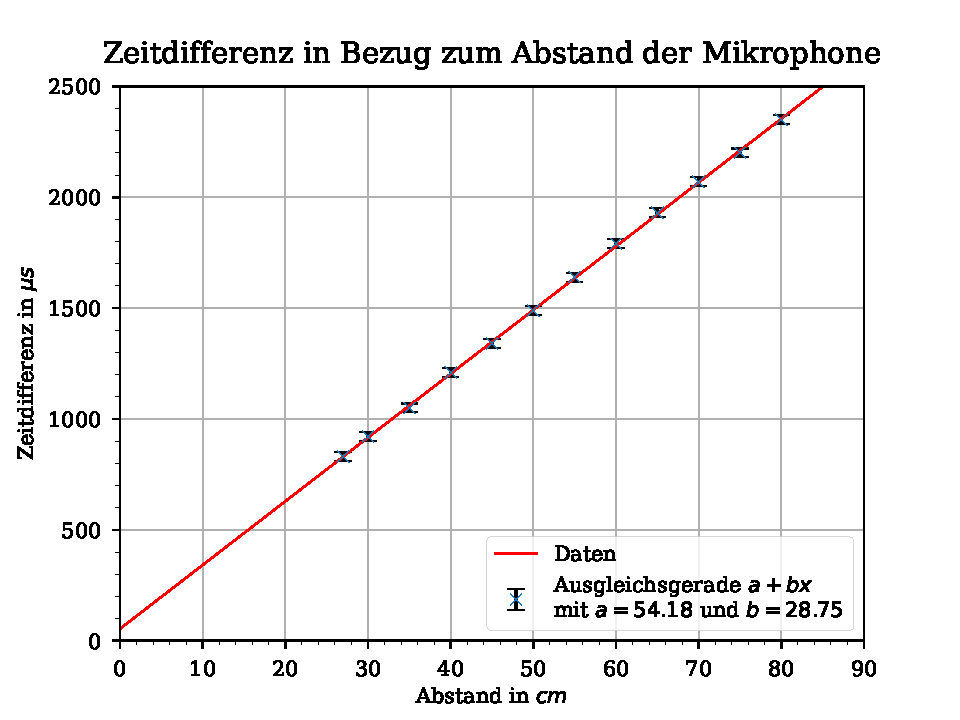
\includegraphics{./2Mikros.pdf}

        \caption{Laufzeitunterschied der Schallwellen}
        \label{fig:graph2}
    \end{figure}
    Im Graph \ref{fig:graph2} sieht man anhand der Steigung die Schallgeschwindigkeit. Man kann erkennen, dass die Ausgleichsgerade nicht durch den Ursprung geht. Das liegt daran,
    dass der Mikrofonabstand systematisch um eine Konstante ($-1,88cm$) abweicht, da die Mikrofone unterschiedlich gebaut und unterschiedlich in die 
    Vorrischtung eingespannt waren. Die Steigung der Ausgleichsgeraden beträgt $28,75\frac{\mu s}{cm}$. Daraus folgt
    dass die Schallgeschwindigkeit
    \begin{align} \label{sch1}
        \nu = \frac{1}{28.75\frac{\mu s}{cm}} = 347.8\frac{m}{s}
    \end{align}
    beträgt. Auch mit dem Literaturwert und der Raumtemeratur von $295,3K$ kann man die Schallgeschwindigkeit
    \begin{align} \label{sch2}
        \nu_T\frac{T}{T_0} = 331,5 \sqrt{\frac{285,3}{273,15}} = 344,8\frac{m}{s}
    \end{align}
    berechnet werden. Diese liegt sehr nahe an der gemessen Schallgeschwindigkeit.

    $\kappa$ kann anhand von $\nu$, dem der Gaskonstante $R = 8,314 \frac{J}{molK}$ der Temperatur $T=295,3$ und der molaren Masse $M=28,96\frac{g}{mol}$ berechnet werden.
    \begin{align}
        \nu = \sqrt{\kappa \frac{RT}{M}} \Rightarrow \kappa = \frac{\nu^2 M}{RT}=1,42
    \end{align}

    \section{Schallgeschwindigkeit mittels stehenden Wellen}

    \subsection{Theorie und experiemteller Aufbau}
    In Aufgabe 3 wird die Phasengeschwindigkeit durch das Erzeugen und Messen 
    einer stehenden Welle in einem Rohr bestimmt, dessen Länge mit einem Stopfen verändert werden kann.
    In dieser überlagern sich die gegeneinander laufenden Wellen,
    die  am Ende vom Stopfen reflektiert werden. Stehende Wellen entstehen nur, wenn das Rohr eine bestimmte Länge hat
    und somit beim am Stopfen ein Knoten und bei der Öffung ein Bauch entsteht, also wenn
    \begin{align} \label{stehwelle}
        l = \frac{2n+1}{4} \lambda = \frac{2n + 1}{4} \cdot \frac{\nu}{f}
    \end{align}
    gilt. Wenn also die Lautstärke im Mikrofon am Rohranfang maximal wird, entsteht dort ein Bauch und die Gleichung
    (\ref{stehwelle}) gilt. Es gilt: 
    \begin{align}
        \Delta l = l_n+1 - l_n &= \frac{2n+3}{4} \lambda - \frac{2n+1}{4} \lambda \nonumber \\
        &= \frac{\nu}{2f} \nonumber \\
         \Rightarrow \nu &= 2f \cdot \Delta l
    \end{align}
    Somit kann mit der Differenz der verschiedenen Rohrlängen, bei denen eine stehende Welle 
    entsteht, die Schallgeschwindigkeit ausgerechnet werden.

    \subsection{Ergebnisse}
    \begin{figure}[h]
        
        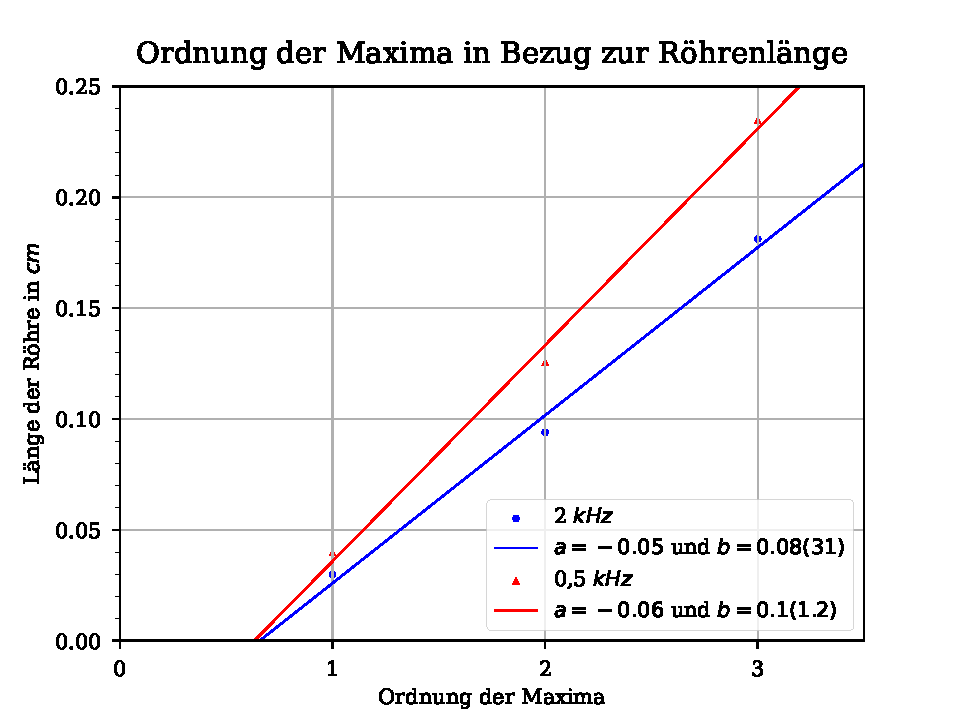
\includegraphics{./Test.pdf}

        \caption{Röhrenlänge bei unterschiedlichen Frequenzen}
        \label{fig:graph3}
    \end{figure}
    Der Graph stellt die Positionen des Stopfen für die Maxima dar. Mit der Steigung kann die Schallgeschwindigkeit
    ausgerechnet werden (Steigung $= \Delta t$ ). Die Unsicherheit der Ausgleichsgeraden wird mithilfe der Formeln im Anhang bestimmt.
    Beim Oszilloskop wurde bei 1kHz eine Schwankung von $\pm 2Hz$, bei $ 2kHz \ \pm 30Hz$ und bei $0.5kHz \ \pm 2Hz $ beobachtet.
  

    \begin{table}
        \centering
        \begin{tabular}[]{c|c|c|c}
            Frequenz & $500(2)Hz$ & $1000(4)Hz$ & $2000(30)Hz$ \\ \hline
            Steigung &  $ 34,4(1,2) \frac{cm}{n}$ & $17,28(71)\frac{cm}{n}$ & $8,56(31)\frac{cm}{n}$ \\ \hline
            Geschwindigkeit & $345,6(14,3) \frac{m}{s}$ & $342,2(13,5) \frac{m}{s}$ & $344,0(12,0)\frac{m}{s}$ 
        \end{tabular}
    \end{table}

    Der gewichtete Mittelwert (Formel siehe Anhang) ist $\bar{x} = 344,03 \frac{m}{s}$. Er hat eine 
    interne Unsicherheit $u_{int} = 0,16\frac{m}{s}$ und eine größere externe und somit Gesamtunsicherheit $u_{ext} = 0,95\frac{m}{s}$.
    Damit stimmt diese Schallgeschwindigkeit mit der in (\ref{sch1}) und der in (\ref{sch2}) überein.


    
   
    \section{Anhang}
    \subsection{Fehlerrechnung}
    \paragraph{Lineare Regression}
    Die Ausgleichsgeraden der Graphen wurden so gezeichnet dass
    \begin{align}
        S=\sum_{i=1}^n(y_i - (a_0 + a_1 x_i))
    \end{align}
    minimal ist. Die Unsicherheit der Steigung $a_1$ lässt sich mit
    \begin{align}
        \sigma_y &= \sqrt{\frac{S}{n-2}} \\
        D &= n \sum_{i=1}^n x_i^2 - \left( \sum_{i=1}^n x_i \right)^2
    \end{align}
    und der Formel
    \begin{align}
        u(a_1) = \sigma_y \sqrt{\frac{n}{D}}
    \end{align}
    berechnen.

    \paragraph{Gewichteter Mittelwert}
    \begin{align}
        \bar{x} = \frac{\sum_{i=1}^n w_i \cdot x_i}{\sum_{i=1}^n w_i} \\
        mit: \ \ w_i = \frac{1}{u(x_i)^2}
    \end{align}

\end{document}